%PAGINA ORIZZONTALE
\newpage
\paperwidth=\pdfpageheight
\paperheight=\pdfpagewidth
\pdfpageheight=\paperheight
\pdfpagewidth=\paperwidth
\headwidth=\textheight

\begingroup 
\vsize=\textwidth
\hsize=\textheight

\subsection{Pianificazione temporale degli incrementi}
\pagestyle{empty}
\begin{figure}[h]
	\centering
	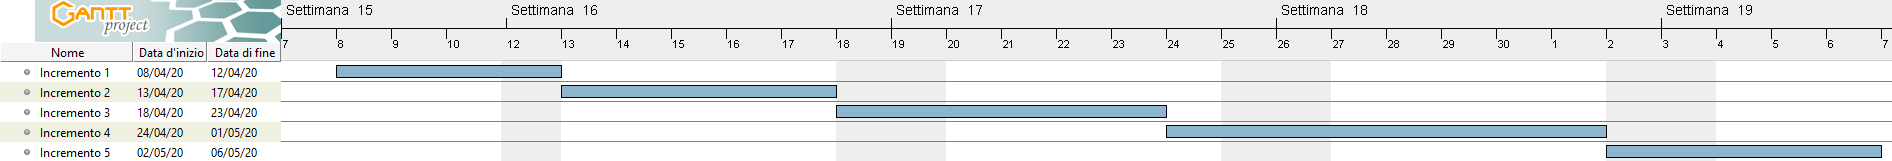
\includegraphics[height = 4cm, width = 24.5cm]{Sezioni/DiagrammiGantt/PianificazioneTemporaleIncrementi.png}
	\caption{Diagramma di Gantt degli incrementi del Periodo 2 della Fase di Progettazione di Dettaglio e Codifica}
\end{figure}

\begin{figure}[h]
	\centering
	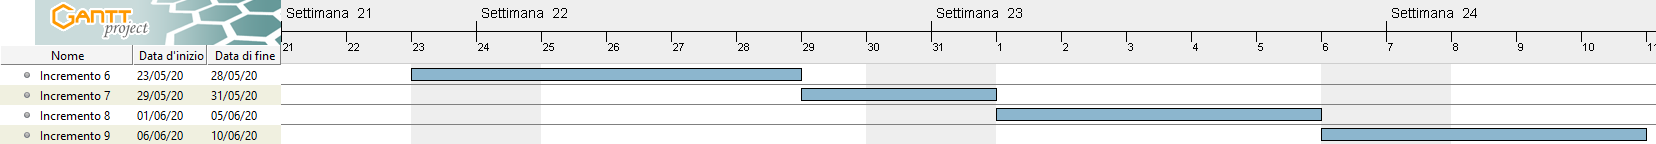
\includegraphics[height = 4cm, width = 24.5cm]{Sezioni/DiagrammiGantt/PianificazioneTemporaleIncrementi2.png}
	\caption{Diagramma di Gantt degli incrementi del Periodo 2 della Fase di Validazione e Collaudo}
\end{figure}

\textwidth=\hsize
\textheight=\vsize

\endgroup
\newpage
\paperwidth=\pdfpageheight
\paperheight=\pdfpagewidth
\pdfpageheight=\paperheight
\pdfpagewidth=\paperwidth
\headwidth=\textwidth